% Packages
\usepackage{graphicx}   % For including graphics (e.g., images)
\usepackage{caption}    % Customizes figure and table captions
\usepackage{marginnote} % For adding margin notes
\usepackage{float}      % Provides the [H] placement option for figures/tables
\usepackage{geometry}   % For setting page margins
\usepackage{xcolor}     % For defining and using colors
\usepackage{tikz}       % For creating graphics and positioning elements
\usepackage{textpos}    % For positioning text blocks
\usepackage{scrlayer-scrpage} % For customizing page headers and footers
\usepackage{etoolbox}   % For programming tools (e.g., hooks, conditionals)
\usepackage[none]{hyphenat} % Disable automatic hyphenation
\usepackage[labelfont=bf, labelsep=colon, format=plain, textfont=bf, justification=raggedright]{caption} % Customize captions
\usepackage{lscape}     % For landscape pages
\usepackage{multicol}
\usepackage{enumitem} % for compact list spacing
\usepackage{calc}
\usepackage{eso-pic} % for AddToShipoutPicture


% Redefine section and subsection commands to adjust heading sizes
\makeatletter
% Section (level 1)
\renewcommand\section{\@startsection{section}{1}{\z@}%
    {-3.5ex \@plus -1ex \@minus -.2ex}% space before
    {2.3ex \@plus .2ex}% space after
    {\Huge\bfseries}}   % Large and bold section headings

% Subsection (level 2)
\renewcommand\subsection{\@startsection{subsection}{2}{\z@}%
    {-3.25ex\@plus -1ex \@minus -.2ex}% space before
    {1.5ex \@plus .2ex}% space after
    {\LARGE\bfseries}}  % Large subsection headings

% Subsubsection (level 3)
\renewcommand\subsubsection{\@startsection{subsubsection}{3}{\z@}%
    {-0.5ex\@plus -0.5ex \@minus -.1ex}% space before
    {0.3ex \@plus 0.1ex}% space after
    {\bfseries}}  % Bold but smaller
\makeatother


%Add a watermark to every page
\AddToHook{shipout/foreground}{
  \begin{tikzpicture}[remember picture,overlay]
    \node[black,rotate=45,scale=6,opacity=0.15] at (current page.center) {Demonstration Only};
  \end{tikzpicture}
}

\usepackage{xcolor}
\usepackage{background}
\usepackage{tikz}
\usepackage{hyperref}

% Define your custom color
\definecolor{stripcolor}{HTML}{1E716F}

% Background setup: 1cm vertical strip on the left side
\backgroundsetup{
  scale=1,
  angle=0,
  opacity=1,
  contents={\rule{1cm}{\paperheight}},
  color=stripcolor,
  position=current page.west,
  vshift=0cm,
  hshift=0.5cm
}
% Custom title page
\makeatletter
\renewcommand{\maketitle}{
  \newpage
  \newgeometry{left=0.65in, right=0.65in, top=1in, bottom=1in}

  \begin{titlepage}
  % Background image
    \begin{tikzpicture}[remember picture,overlay]
      \node[anchor=north east, xshift=4cm, opacity=1] at (current page.north east)
        {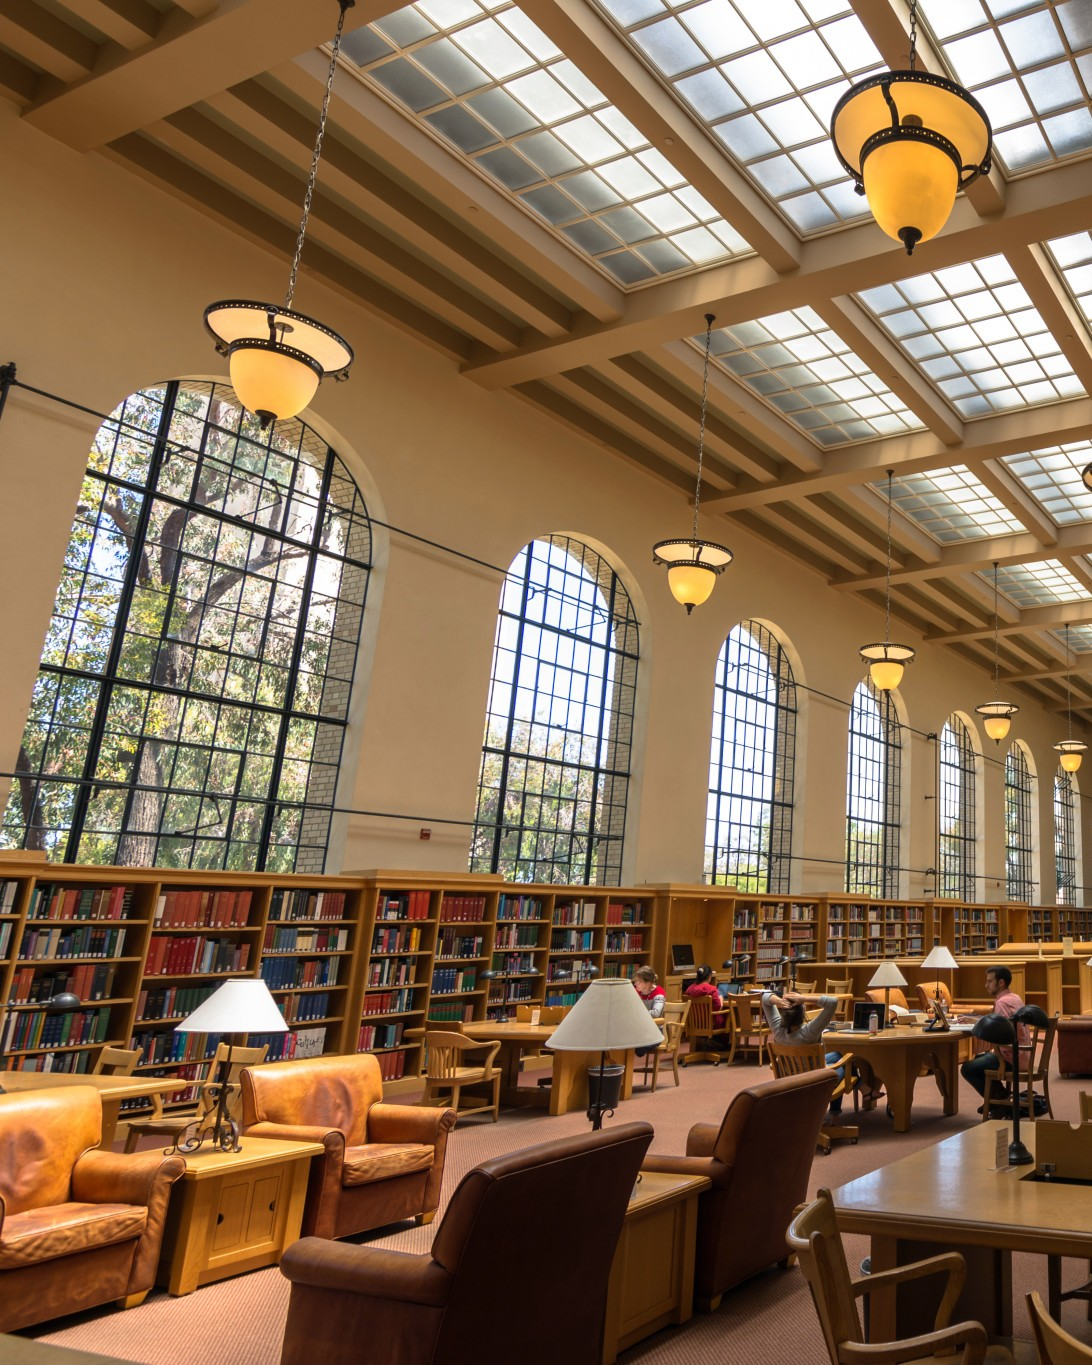
\includegraphics[height=13in]{../fig/library.jpg}};
    \end{tikzpicture}
    

    % --- Top white strip with title/subtitle (drawn after image!) ---
    \begin{tikzpicture}[remember picture,overlay]
      \node[anchor=north west, fill=white, minimum width=\paperwidth, 
            minimum height=3cm, inner sep=15pt] 
        (headerbox) at (current page.north west) {};

      % Title + subtitle inside the strip
      \node[anchor=west, xshift=5cm, yshift=-1.5cm, align=left] 
        at (headerbox.north west) {
          \Huge\bfseries \@title \\[4pt]
          \Large\bfseries \@subtitle
        };
        
      % Date on the right
      \node[anchor=east, xshift=-2cm, yshift=-1.5cm, align=right] 
        at (headerbox.north east) {
          \Large \@date 
        };

      % Logo over the strip
      \node[anchor=north west, xshift=0.65in, yshift=-.1cm] 
        at (current page.north west) 
        {
\includegraphics[height=2.5cm]{../fig/bob_loblaw.jpg}};
    \end{tikzpicture}

    % --- Bottom white strip ---
    \begin{tikzpicture}[remember picture,overlay]
      \node[anchor=south west, fill=white, minimum width=\paperwidth, 
            minimum height=2.5cm, inner sep=15pt] 
        (footerbox) at (current page.south west) {};

      % Contact info (bottom left)
      \node[anchor=south west, xshift=0.65in, yshift=0.5cm, align=left] 
        at (footerbox.south west) {
          \Large\textbf{\@author} \\[-2pt]
          \normalsize\href{mailto:dallasnovakowski@gmail.com}{dallasnovakowski@gmail.com} \\[-2pt]
          \normalsize\url{https://dallasnova.rbind.io}
        };

      % Logos (bottom right)
      \node[anchor=south east, xshift=-1cm, yshift=0.17cm] 
        at (footerbox.south east) {
          
\includegraphics[height=1.7cm]{../fig/socia_logo.png}
        };
    \end{tikzpicture}


    % Vertical strip over the image
    \begin{tikzpicture}[remember picture,overlay]
      \fill[stripcolor, opacity=1] (current page.north west) rectangle ++(1cm,-\paperheight);
    \end{tikzpicture}


  \end{titlepage}
  \restoregeometry
}
\makeatother


\makeatletter
\AddToHook{shipout/foreground}{%
  \ifnum\value{page}>1 % <- only apply after page 1
    \begin{tikzpicture}[remember picture,overlay]
      \node[anchor=north, xshift=-3cm, yshift=-.5cm] at (current page.north east)
        {
\includegraphics[height=1.5cm]{../fig/bob_loblaw.jpg}};
      % Header - logo
      \node[anchor=south, xshift=11cm, yshift=.3cm] at (current page.south west)
        {
\includegraphics[width=3cm]{../fig/socia_logo.png}};
      % Footer text (left)
      \node[anchor=north, yshift=-1cm] at (current page.north) {\@title};

      % Optional subtitle
      %\node[anchor=north west, xshift=2cm, yshift=-1.5cm] at (current page.north west)
       % {\scriptsize $subtitle$};
      % Page number (right)
      \node[anchor=south east, xshift=-1.7cm, yshift=.8cm] at (current page.south east)
        {\footnotesize \pagemark};
    \end{tikzpicture}%
  \fi
}
\makeatother


% Set margins for the rest of the document
\newgeometry{left=0.65in, right=3.3in, top=1in, bottom=1in}

% Use custom fonts
\setsansfont{OpenSans}[
    Path=OpenSans/,
    Scale=0.9,
    Extension = .ttf,
    UprightFont=*-Regular,
    BoldFont=*-Bold,
    ItalicFont=*-Italic,
    ]
\setmainfont{OpenSans}[
    Path=OpenSans/,
    Scale=0.9,
    Extension= .ttf,
    UprightFont=*-Regular,
    BoldFont=*-Bold,
    ItalicFont=*-Italic,
    ]

% Redefine figure and table names
\renewcommand{\figurename}{\MakeUppercase{\bfseries FIGURE}}
\renewcommand{\tablename}{\MakeUppercase{\bfseries TABLE}}




% Adjust margin note settings
% 
\pretocmd{\marginnote}{\raggedright}{}{}
% \setlength{\marginparwidth}{2.4in} % Width of the margin notes
\setlength{\marginparwidth}{2.6in} % Width of the margin notes

\setlength{\marginparsep}{3em}     % Separation between margin notes and main text
\setlength{\marginparpush}{1em}    % Space between consecutive margin notes


\newlength{\fullwidthwithmargin}
\setlength{\fullwidthwithmargin}{\textwidth}
\addtolength{\fullwidthwithmargin}{\marginparwidth}



\newcounter{customfigure}

% 
% \newcommand{\figuremarginnote}[2]{%
%   \refstepcounter{customfigure}
%   \addcontentsline{lof}{figure}{\textbf{\thecustomfigure \hspace{\fontdimen2\font} \hspace{\fontdimen2\font}}     #1}
%   \footnotesize{\marginnote{\parbox{\marginparwidth  - \marginparsep}{\textbf{\MakeUppercase{FIGURE} \thecustomfigure: }#1 \vspace{0.5em} \\ \raggedright{\textit{#2}}}}}%
% }
% 
% 
% \newcommand{\figuremarginnote}[2]{%
%   \refstepcounter{customfigure}
%   \addcontentsline{lof}{figure}{\textbf{\thecustomfigure \hspace{\fontdimen2\font} \hspace{\fontdimen2\font}}     #1}
%   \footnotesize{\marginnote{%
%     \parbox{\marginparwidth - \marginparsep}{%
%       \textbf{\MakeUppercase{FIGURE} \thecustomfigure: }#1%
%       \vspace{0.5em} \\
%       \colorbox{gray!5}{%
%         \parbox{\dimexpr\marginparwidth - \marginparsep - 2\fboxsep}{%
%           \raggedright\textit{#2}%
%         }%
%       }%
%     }%
%   }}%
% }
% 


\setlength{\fboxsep}{5pt}  % or any value you prefer

\newcommand{\figuremarginnote}[2]{%
  \refstepcounter{customfigure}
  \addcontentsline{lof}{figure}{\textbf{\thecustomfigure \hspace{\fontdimen2\font} \hspace{\fontdimen2\font}}     #1}
  \footnotesize{\marginnote{%
    \parbox{\marginparwidth - \marginparsep}{%
      \raggedright
      \textbf{\MakeUppercase{FIGURE} \thecustomfigure: }#1%
      \vspace{0.5em} \\
      \colorbox{gray!5}{%
        \parbox{\dimexpr\marginparwidth - \marginparsep - 2\fboxsep}{%
          \raggedright\textit{#2}%
        }%
      }%
    }%
  }}%
}

\newcommand{\figurecaption}[1]{%
  \refstepcounter{customfigure}
  \addcontentsline{lof}{figure}{\textbf{\thecustomfigure \hspace{\fontdimen2\font} \hspace{\fontdimen2\font}}     #1}
  \footnotesize{\textbf{\MakeUppercase{FIGURE} \thecustomfigure: }#1}
}

\newcommand{\lowerfigurenote}[2]{%
  \refstepcounter{customfigure}
  \addcontentsline{lof}{figure}{\textbf{\thecustomfigure \hspace{\fontdimen2\font} \hspace{\fontdimen2\font}}#1}
  \footnotesize\begin{textblock*}{\marginparwidth - \marginparsep}(1.06\textwidth,22em) % Adjust position (0.9\textwidth shifts to the right, 1pt adjusts vertical position)
    \footnotesize\parbox{\marginparwidth}{%
      \textbf{\MakeUppercase{FIGURE} \thecustomfigure: }#1\vspace{.5em}\\%
      \raggedright{\textit{#2}}%
    }%
  \end{textblock*}
}



\newcounter{customtable}


\newcommand{\tablemarginnote}[2]{%
  \refstepcounter{customtable}
  \addcontentsline{lot}{table}{\textbf{\thecustomtable \hspace{\fontdimen2\font} \hspace{\fontdimen2\font}}     #1}
  \footnotesize\marginnote{\parbox{\marginparwidth}{\textbf{\MakeUppercase{TABLE} \thecustomtable: }#1 \vspace{0.5em} \\ \raggedright{\textit{#2}}}}%
}

% \newcommand{\rrmargintext}[1]{%
%   \marginnote{%
%     \parbox{\marginparwidth - \marginparsep}{%
%       \raggedright\textit{#1}%
%     }%
%   }%
% }


\newcommand{\rrmargintext}[1]{%
  \marginnote{%
    \colorbox{gray!5}{%
      \parbox{\dimexpr\marginparwidth - \marginparsep - 2\fboxsep}{%
        \raggedright\textit{#1}%
      }%
    }%
  }%
}

\newcommand{\tablecaption}[1]{%
  \refstepcounter{customtable}
  \addcontentsline{lot}{table}{\textbf{\thecustomtable \hspace{\fontdimen2\font} \hspace{\fontdimen2\font}}     #1}
  \textbf{\MakeUppercase{TABLE} \thecustomtable: }#1
}
%


\newcommand{\sdossfig}[5]{%
  \figuremarginnote{#1}{%
    #2
    \newline
    {\noindent\rule{\dimexpr\marginparwidth - \marginparsep - #3\fboxsep\relax}{0.4pt}}
    (n = #4) \quad \underline{PROMPT:} #5
  }
}



\newcommand{\sdossfiga}[5]{%
  \begin{figure}[htbp]
    \centering
    \includegraphics[width=\textwidth]{#1}
    \caption{#2 \newline (n = #4) \quad \underline{PROMPT:} #5}
    \label{fig:#1}
  \end{figure}
  \figuremarginnote{#2}{%
    #3 \newline
    {\noindent\rule{\dimexpr\marginparwidth - \marginparsep - 2\fboxsep\relax}{0.4pt}} % Fixed rule width
    (n = #4) \quad \underline{PROMPT:} #5
  }
}


\pagestyle{empty}  % Start with no default header/footer
